\documentclass[Interploate_hadwritten_Digits.tex.tex]{subfiles}

\begin{document}
	\subsection{Aufbereitung der Daten}
	Als Datensatz wurde der MNIST Datensatz von der offiziellen Webseite\footnote{ http://yann.lecun.com/exdb/mnist/} von Yann LeCun verwendet. Dieser Umfasst ein Trainingsset von \numprint{60000} und ein Testset von \numprint{10000} gelabelten Datensätzen in jeweils zwei verschiedenen Dateien, eine für die Bilder und eine für die Labels. Von der Bilder-Datei werden die jeweils 28x28 Bytes eingelesen und in einen 784-dimensionalen Vektor eingelesen. Dabei werden die Werte auf Float-Werte zwischen Null und Eins verwandelt. Die Label-Datei wird Byteweise eingelesen und in eine One-Hot Vektor der Länge zehn verwandelt, bei welchem der Index der Eins dem Wert des Labels entspricht. 
	
	\subsection{Trainieren des Neuronalen Netzes}
	Das Neuronale Netz wurde mit Tensorflow\footnote{https://www.tensorflow.org} modelliert und trainiert. Das verwendete Modell ist ein Feed Forward Neuronal Network mit Weights und Biases für jede Schicht. Um den Output des Netzes zu berechnen, muss $ \vec{x_{n}} $ berechnet werden, wobei $ x_{0} $ dem Bildvektor entspricht und die restlichen Werte gemäss Formel \ref{eq:layer_calculation} berechnet werden. $ n $ entspricht dabei der Anzahl Schichten im Neuronalen Netz.
	\begin{equation}
	\vec{x_{i}} = a(\vec{x_{i-1}} \times w_{i-1} + b_{i-1})
	\label{eq:layer_calculation}
	\end{equation}
	Als Aktivierungsfunktion $ a(x) $ wird die Logistische Sigmoidfunktion (siehe Gleichung \ref{eq:sigmoid}) verwendet, welche auf alle Elemente im Vektor angewendet wird. 
	\begin{equation}
	f(x)=\frac{1}{1+e^{-x}}
	\label{eq:sigmoid}
	\end{equation}
	Sie hat die Aufgabe zu verhindern, dass Zahlen durch die Multiplikationen zu gross oder zu klein werden. Dieses Verhalten wurde in der Abbildung \ref{fig:sigmoid_plot} visualisiert.
	\begin{Figure}
		\centering
		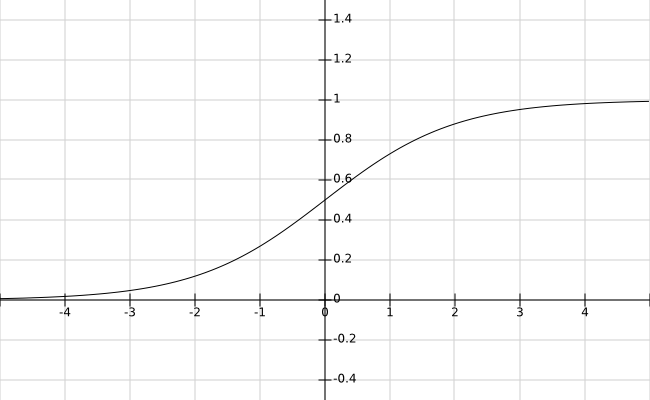
\includegraphics[width=\linewidth]{img/sigmoid_plot.png}
		\captionof{figure}{Verhalten der Sigmoid Funktion}
		\label{fig:sigmoid_plot}
	\end{Figure}
	
	\subsection{Rückrechnung im Neuronalen Netz}
	
	\subsection{Approximation von Input Bildern}
	
\end{document}